\documentclass[a4paper,12pt]{article}
\usepackage{amsmath}
\usepackage{amssymb}
\usepackage[polish]{babel}
\usepackage{polski}
\usepackage[utf8]{inputenc}
\usepackage{indentfirst}
\usepackage{geometry}
\usepackage{array}
\usepackage[pdftex]{color,graphicx}
\usepackage{subfigure}
\usepackage{afterpage}
\usepackage{setspace}
\usepackage{color}
\usepackage{wrapfig}
\usepackage{listings}
\usepackage{datetime}

\renewcommand{\onehalfspacing}{\setstretch{1.6}}

\geometry{tmargin=2.5cm,bmargin=2.5cm,lmargin=2.5cm,rmargin=2.5cm}
\setlength{\parindent}{1cm}
\setlength{\parskip}{0mm}

\newenvironment{lista}{
\begin{itemize}
  \setlength{\itemsep}{1pt}
  \setlength{\parskip}{0pt}
  \setlength{\parsep}{0pt}
}{\end{itemize}}

\newcommand{\linia}{\rule{\linewidth}{0.4mm}}

\definecolor{lbcolor}{rgb}{0.95,0.95,0.95}
\lstset{
    backgroundcolor=\color{lbcolor},
    tabsize=4,
  language=C++,
  captionpos=b,
  tabsize=3,
  frame=lines,
  numbers=left,
  numberstyle=\tiny,
  numbersep=5pt,
  breaklines=true,
  showstringspaces=false,
  basicstyle=\footnotesize,
  identifierstyle=\color{magenta},
  keywordstyle=\color[rgb]{0,0,1},
  commentstyle=\color{Darkgreen},
  stringstyle=\color{red}
  }

\begin{document}

\noindent
\begin{tabular}{|c|p{11cm}|c|} \hline 
Grupa 6 & Wojciech Król, Maciej Kieruczenko & \ddmmyyyydate\today \tabularnewline
\hline 
\end{tabular}


\section*{Zadanie 2 - Wyznacznik macierzy - GPU}

Ćwiczenie polegało na policzeniu wyznacznika zadanej w parametrze wywołania macierzy przy pomocy biblioteki CUDA. Mierzony był czas wykonywanych obliczeń, który zmieniał się wraz z kolejnymi wątkami.

Według definicji wyznacznik macierzy jest unikalną liczbą, która jest przyporządkowywana macierzy kwadratowej. W programie skorzystano z rozkladu LU, dzięki któremu wyznacznik można wyliczyć przy pomocy wzoru: $det(A)=det(L*U)=det(L)*det(U)$ (co jest równe sumie elementów na przekątnej macierzy U: $\sum_{i=0}^{n-1} u_{i,i}$), gdzie L to macierz dolna, a U macierz górna. 

Poniżej znajduje się część kodu programu wykonywana równolegle:

\begin{lstlisting}
__global__ void decompositionKernelNew(double *deviceMtrx, int mtrxSize, int idx, int maxIndex)
{
    int tid = threadIdx.x + blockIdx.x * blockDim.x;
    while (tid < maxIndex)
    {
        int startIdx = ((idx + tid + 1) * mtrxSize + idx);
        int endIdx = ((idx + tid + 1) * mtrxSize + mtrxSize);
        for (int i = startIdx + 1; i < endIdx; i++)
        {
            deviceMtrx[i] = deviceMtrx[i]-(deviceMtrx[startIdx] * deviceMtrx[(idx * mtrxSize)+(idx + (i - startIdx))]);
        }
        tid += blockDim.x * gridDim.x; 
    }
}
\end{lstlisting}

Do otrzymania bieżącej wartości zmiennej \textit{tid} wykorzystywany jest indeks aktualnego wątku, bloku oraz liczba wątków przyporządkowanych do tego bloku. Następnie na podstawie tych danych wykonywane są kolejne operacje dekompozycji macierzy na GPU. Powyższy kod funkcji jest wywoływany w następujący sposób:

\begin{lstlisting}
decompositionKernelNew <<<blockCount, threadCount>>>(deviceMtrx, mtrxSize, idx,mtrxSize - idx - 1);
\end{lstlisting}

Testy były wykonywane na macierzy 1000x1000. Liczbę bloków ustalono na 10. Wyliczony wyznacznik macierzy wyniósł $-7.12832e+13$. Wyniki zestawiono w postaci dwóch wykresów - zależności czasu obliczeń oraz przyspieszenia od liczby wątków. Dodatkowo należy wspomnieć, że ze względu na brak wykorzystania pamięci współdzielonej i synchronizacji sposób podziału na gridy/bloki jest nie istony - ważna jest jedynie sumaryczna liczba wątków.

\begin{figure}[!h]
	\centering
  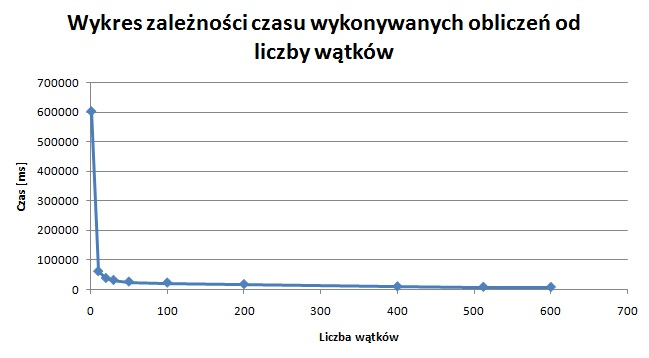
\includegraphics[width=0.6\textwidth]{1.jpg}
\end{figure}

\begin{figure}[!h]
	\centering
  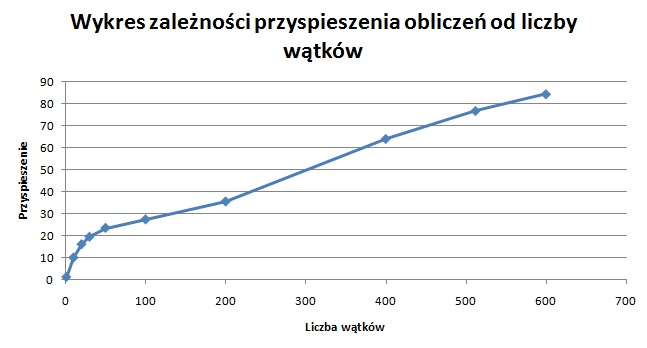
\includegraphics[width=0.6\textwidth]{2.jpg}
\end{figure}

\vspace{10cm}
Na podstawie powyższych wykresów można stwierdzić, że wyniki pomiaru czasu obliczeń są zgodne z oczekiwanymi. Dla niewielkiej ilości wątków wzrost przyspieszenia był bardzo gwałtowny, zaś poczynając od ok. 50 wątków zaczął się stabilizować na stałym poziomie. Dzieje się tak z powowodu nierównomiernego rozłożenia pracy między poszczególne wątki.

\vspace{1cm}
Wnioski z wykonywanego ćwiczenia:
\begin{lista}
\item Dzięki zastosowaniu technologii CUDA można znacząco przyspieszyć czas obliczeń wyznacznika dużych macierzy (dla niewielkich pojedynczy wątek CPU będzie szybszy),
\item Większość algorytmów obliczania wyznacznika jest trudna do zrównoleglenia w swojej podstawowej postaci (nowe wartości wyliczane są na podstawie poprzednio wyliczonych wartości sąsiadujących elementów macierzy) ,
\item Najlepsze wyniki osiągnięto dla łącznej ilości wątków zbliżonej liczbie jednostek obliczeniowych karty graficznej.
\end{lista}

\end{document}
